\documentclass[10pt]{article}
\usepackage[utf8]{inputenc}
\usepackage[italian]{babel}
\usepackage{multicol}
\usepackage[a4paper, total={18cm, 25cm}]{geometry}
\usepackage{listings}
\usepackage{graphicx}
\graphicspath{ {./img/} }
\begin{document}
\title{Reti di Calcolatori e Laboratorio}
\author{Federico Matteoni}
\date{ }
\renewcommand*\contentsname{Indice}

\maketitle
\tableofcontents
\pagebreak
\section{Introduzione}
Appunti del corso di \textbf{Reti di Calcolatori} presi a lezione da \textbf{Federico Matteoni}.\\\\
Prof.: \textbf{Federica Paganelli}, federica.paganelli@unipi.it\\
\begin{list}{-}{Riferimenti web:}
\item \emph{elearning.di.unipi.it/enrol/index.php?id=169}\\Password: \textbf{RETI2019}
\end{list}
Esame: scritto (o compitini), discussione orale facoltativa + progetto con discussione (progetto + teoria di laboratorio, progetto da consegnare 7gg prima della discussione)\\
\begin{list}{-}{Libri e materiale didattico:}
\item Slide su eLearning
\item IETF RFC\\tools.ietf.org/rfc\\www.ietf.org/rfc.html
\item "Computer Networks: A Top-Down Approach" B. A. Forouzan, F. Mosharraf, McGraw Hill
\end{list}
Ricevimento: stanza 355 DO, II piano

\section{Rete}
\paragraph{Definizione di rete} Interconnessione di dispositivi in grado di scambiarsi informazioni, come end system, router, switch e modem.\\
\begin{list}{}{Gli end system possono essere di due tipi:}
\item \textbf{Host}: una macchina, in genere di proprietà degli utenti, \textbf{dedicata ad eseguire applicazioni}. Esempi: desktop, portatile, smartphone, tablet\ldots
\item \textbf{Server}: una macchina, tipicamente con elevate prestazioni, destinata ad eseguire programmi che \textbf{forniscono servizi} a diverse applicazioni utente. Esempi: posta elettronica, web, \ldots
\end{list}
\textbf{Con il termine host si può anche indicare un server}.

\subsection{Tipi di Rete}
\paragraph{Local Area Network} Una \textbf{LAN è una rete di area geografica limitata}: un ufficio, una casa ecc.. I dispositivi comunicano attraverso una determinata tecnologica: switch, BUS, HUB ecc..\\
In una rete locale tipicamente una serie di host comunicano tra loro attraverso, ad esempio, uno switch centrale.
\paragraph{Wide Area Network} Alcuni esempi:\\
\begin{multicols}{2}
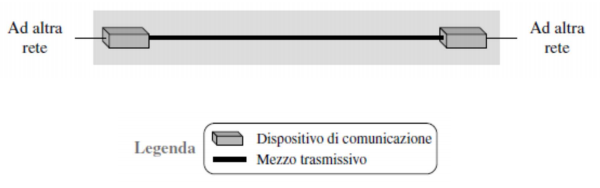
\includegraphics[scale=0.5]{wan1.png}\\
\columnbreak
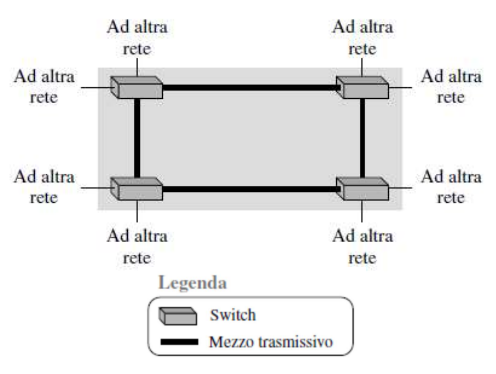
\includegraphics[scale=0.5]{wan2.png}\\
\end{multicols}

\subsection{Internetwork}
Una \textbf{internetwork} si crea quando si \textbf{interconnettono diverse reti}.
Alcuni esempi:\\
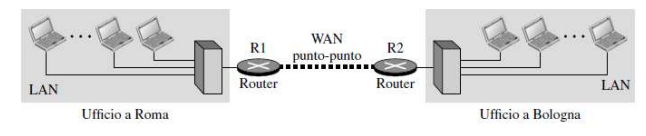
\includegraphics[scale=1]{internetwork1.png}\\
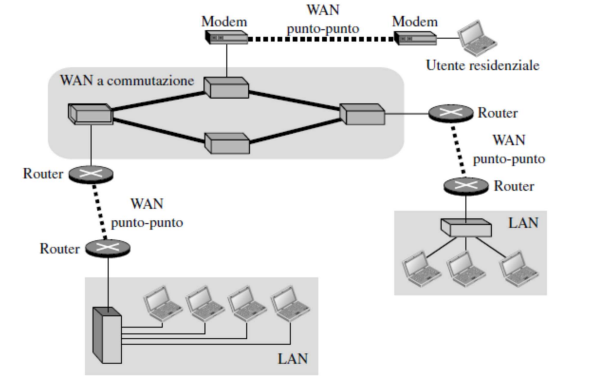
\includegraphics[scale=0.75]{internetwork2.png}\\

\subsection{Switching}
Una rete internet è formata dall'interconnesione di reti composte da link e dispositivi capaci di scambiarsi informazioni.
In particolare, i sistemi terminali comunicano tra di loro per mezzo di dispositivi come switch, router ecc. che si trovano nel percorso tra i sistemi sorgente e destinazione.
\paragraph{Switched Network} Reti a commutazione di circuito, tipico delle vecchie reti telefoniche\\
Le risorse sono riservate end-to-end per una connessione. Le risorse di rete (es. bandwidth) vengono suddivise in pezzi, e ciascun pezzo è allocato ai vari collegamenti. Le risorse rimangono inattive se non vengono utilizzate, cioè \textbf{non c'è condivisione}. L'allocazione della rete rende necessario un setup della comunicazione.\\A tutti gli effetti vi è un circuito dedicato per tutta la durata della connessione. Ciò è rende poco flessibile l'utilizzo delle risorse (\textbf{overprovisioning}).
\paragraph{Packet-Switched Network} Reti a commutazione di pacchetto, più moderno\\
Flusso di dati punto-punto suddiviso in pacchetti. I pacchetti degli utenti condividono le risorse di rete. Ciascun pacchetto utilizza completamente il canale.\\\textbf{Store and Forward}: il commutatore deve ricevere l'intero pacchetto prima di ritrasmetterlo in uscita.\\Le risorse vengono usate \textbf{a seconda delle necessità}. Vi è \textbf{contesa per le risorse}: la richiesta di risorse può eccedere la disponibilità e si può verificare \textbf{congestione} quando i pacchetti vengono accodati in attesa di utilizzare il collegamento. Si possono anche verificare perdite.
\section{Internet} L'internetwork più famosa ed utilizzata è \textbf{internet}, ed è composta da migliaia di reti interconnesse. \textbf{Ogni rete} connessa ad internet \textbf{deve utilizzare il protocollo IP} e rispettare certe convenzioni su nomi ed indirizzi. Si possono aggiungere nuove reti ad internet molto facilmente.
\paragraph{Dispositivi in internet} I \textbf{dispositivi} connessi ad internet possono essere host, end systems come PC, workstations, servers, pda, smartphones ecc\ldots\\
I \textbf{link di comunicazione} possono essere fibre ottiche, doppini telefonici, cavi coassiali, onde radio\ldots
Le \textbf{entità software} in internet possono essere:
\begin{list}{}{}
\item \textbf{Applicazioni} e processi
\item \textbf{Protocolli}: regolamentano la trasmissione e la ricezione di messaggi (TCP, IP, HTTP, FTP, PPP\ldots)
\item \textbf{Interfacce}
\item \textbf{Standard} di internet e del web: RFC (Request for Comments) e W3C.
\end{list}
\textbf{Internet è una visione dei servizi}. L'infrastruttura di comunicazione permette alle applicazioni distribuite di scambiare informazioni (WWW, e-mail, giochi, e-commerce, controllo remoto\ldots) e fornisce loro \textbf{servizi di comunicazione connectionless} (senza garanzia di consegna) o \textbf{connection-oriented} (dati garantiti in integrità, completezza ed ordine).
\subsection{Enti Ufficiali} L'\textbf{Internet Engineering Task Force} (IETF) è l'organismo che studia e sviluppa i protocolli in uso su internet. Si basa su gruppi di lavoro a cui chiunque può accedere. I documenti ufficiali che pubblica, dove descrivono i protocolli usati in internet, sono gli RFC/STD (Request for Comments/STanDards).\\
L'\textbf{Internet Corporation for Assigned Names and Numbers} (ICANN) si occupa di coordinare il sistema dei \textbf{nomi di dominio} (DNS) e assegna i gruppi di indirizzi, gli identificativi di protocollo.\\\\
\begin{center}
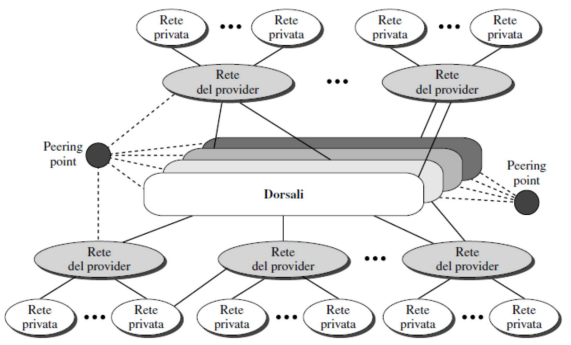
\includegraphics[scale=1]{internet.png}\\
\textbf{Peering point}: interconnessione tra due sistemi autonomi\\
\end{center}
\pagebreak
\subsection{Reti di accesso} Il collegamento tra l'utente ed il primo router di internet è detto \textbf{rete di accesso}.
\begin{list}{}{Può avvenire in 3 modi:}
\item \textbf{Tramite rete telefonica}: servizio dial-up, ADSL\ldots
\item \textbf{Tramite reti wireless}
\item \textbf{Collegamento diretto}, come collegamenti WAN dedicati ad alta velocità (aziende e università)
\end{list}
\section{Metriche di Riferimento}
Come misurare le prestazioni della rete?
\begin{list}{}{Tramite una serie di metriche:}
\item \textbf{Bandwith} o ampiezza di banda: è la larghezza dell'intervallo di frequenze utilizzato dal sistema trasmissivo (Hz).\\\textbf{Bitrate} o \textbf{transmission rate}: quantità di bit che possono essere trasmessi o ricevuti nell'unità di tempo (bit/secondo, bps)\\Il bitrate dipende dalla bandwidth e dalla tecnica trasmissiva utilizzata.
\item \textbf{Throughput}: la quantità di traffico che arriva realmente a destinazione nell'unità di tempo (al netto di perdite sulla rete, funzionamento dei protocolli ecc\ldots).\\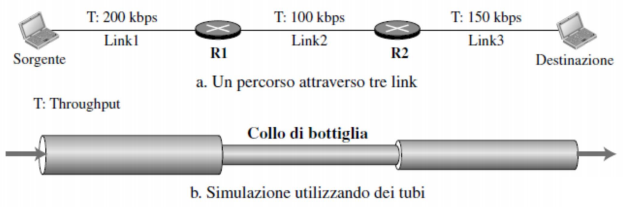
\includegraphics[scale=1]{throughput.png}\\Non è detto che corrisponda alla bandwidth perché ci potrebbe essere un collo di bottiglia.
\item \textbf{Latenza} o ritardo: il tempo richiesto affinché un messaggio arrivi a destinazione dal momento in cui il primo bit parte dalla sorgente.\\
\texttt{latenza = ritardo di propagazione + ritardo di trasmissione + ritardo di accodamento + ritardo di elaborazione}
\item \textbf{Perdita di pacchetti}. Come si può verificare?\\
\begin{multicols}{2}
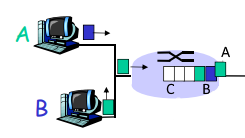
\includegraphics[scale=1]{ritpackets.png}\\

\columnbreak
A $\rightarrow$ pacchetti \textbf{in attesa} di essere trasmessi (\emph{ritardo})\\
B $\rightarrow$ pacchetti \textbf{accodati} (\emph{ritardo})\\
C $\rightarrow$ buffer \textbf{liberi} (se non ci sono buffer liberi, i pacchetti in arrivo vengono scartati, \emph{perdita})\\\\
I pacchetti da spedire vengono accodati nei buffer dei router. Di solito, il tasso di arrivo dei pacchetti sul router eccede le capacità del router di evaderli, quindi \textbf{i pacchetti si accodano in attesa del proprio turno}.
\end{multicols}
Il \textbf{ritardo di elaborazione} è dato dal controllo sui bit e dalla determinazione del canale di uscita (trascurabile)\\
Il \textbf{ritardo di accodamento} è dato dall'attesa di un pacchetto di essere trasmesso (B)\\
Il \textbf{ritardo di trasmissione} è il tempo impiegato per trasmettere un pacchetto sul link.\\\texttt{R$_{trasmissione}$ = R/L}\\
\texttt{R} = rate di trasmissione del collegamento, in bps\\
\texttt{L} = lunghezza del pacchetto in bit\\
Il \textbf{ritardo di propagazione} è il tempo impiegato da 1 bit per essere propagato da un nodo all'altro.\\\texttt{R$_{propagazione}$ = d/s}\\
\texttt{d} = lunghezza del collegamento\\
\texttt{s} = velocità di propagazione del collegamento (si usa la velocità della luce, circa 3 x 10$^{8}$ m/s)
\end{list}
\texttt{d$_{nodal}$ = d$_{proc}$ + d$_{queue}$ + d$_{trans}$ + d$_{prop}$}\\
\texttt{d$_{proc}$} = \textbf{ritardo di elaborazione}, pochi microsecondi\\
\texttt{d$_{queue}$} = \textbf{ritardo di accodamento}, dipende dalla congestione\\
\texttt{d$_{trans}$} = \textbf{ritardo di trasmissione}, \texttt{L/R} e significativo a lunga distanza\\
\texttt{d$_{prop}$} = \textbf{ritardo di propagazione}, \texttt{d/s}, da pochi microsecondi a centinaia di millisecondi\\
\section{Modelli Stratificati}
$https://elearning.di.unipi.it/pluginfile.php/27387/mod_resource/content/1/L02_introduzione_protocolli.pdf$
\paragraph{Perché usare un modello a strati} Per mandare dei dati da un host ad un altro comunicando su una rete, si devono eseguire una \textbf{serie di operazioni}: \textbf{trovare il percorso} di rete da attraversare, \textbf{decidere in che modo spedire e codificare} i dati, \textbf{risolvere eventuali problemi} di comunicazione e altro ancora.\\
Programmare ogni volta tutto il procedimento è un \textbf{lavoro estremamente complesso} e ripetitivo. Un modello a strati \textbf{astrae su più livelli il problema della trasmissione dati} in modo da fornire di volta in volta strumenti utili al programmatore per poter evitare di "\textit{reinventare la ruota}".
\paragraph{Definizioni generali} Nelle architetture di comunicazione a strati sono importanti una serie di definizioni:
\begin{list}{-}{}
\item Stratificazione
\item Information hiding
\item Separation of concern
\item Modello ISO/OSI
\item Stack TCP/IP
\end{list}
Tali definizioni verranno viste durante il corso.
\paragraph{Lo Strato} Uno \textbf{strato} è un \textbf{modulo interamente definito} attraverso i servizi, le interfacce e i protocolli che lo caratterizzano. Si indica anche col nome di livello.\\
Uno strato \texttt{n} \textbf{comunica direttamente} con lo strato \texttt{n} di un'altra unità tramite un \textbf{protocollo assegnato}. Lo stesso strato \texttt{n} può richiedere servizi allo strato \texttt{n-1} attraverso la \textbf{loro interfaccia}, e fornisce servizi allo strato \texttt{n+1} attraverso la \textbf{rispettiva interfaccia}.
\paragraph{Es. modello stratificato: sistema postale}\texttt{Vedi slide\\$https://elearning.di.unipi.it/pluginfile.php/27387/mod_resource/content/1/L02_introduzione_protocolli.pdf$, 48}\\
Dal livello più alto al livello più basso per la spedizione, viceversa per la ricezione. Un problema importante che si incontra quando si manda una lettera, ad esempio, dall'Italia al Giappone è la traduzione. In una \textbf{serie di passi}, in cui in ognuno viene \textbf{eseguito un particolare compito su un messaggio}, che viene poi \textbf{trasferito ad un altro livello}. Nell'esempio, la segretaria prepara lettera (traduce in giapponese e imbusta) affinché il postino la possa prendere. Però il "messaggio" della segretaria è "scritto" per essere interpretato dalla segretaria giapponese, il direttore italiano scrive per il direttore giapponese. \textbf{Messaggi di un livello del sistema che spedisce sono scritti per essere interpretati dal medesimo livello del sistema ricevente}.
\subsection{Perché stratificare} La stratificazione è molto utile per \textbf{scomporre il sistema complesso della gestione della comunicazione}. Prendo un sistema estremamente costoso da costruire per una singola coppia di aziende, quindi lo trasformo in strati così che il costo della singola lettera sia irrisorio.\\
\textbf{Definisco funzioni di base per effettuare trasferimento e agenti che le svolgono}.
\begin{list}{}{Principi di base:}
\item \textbf{Separation of Concern}\\\textbf{Far fare} ad un determinato strato \textbf{solo ciò che gli compete}, \textbf{delegando agli altri tutto ciò che è delegabile}
\item \textbf{Information Hiding}\\\textbf{Nascondo} ad un determinato strato \textbf{le informazioni non indispensabili allo svolgere della sua operazione}.
\end{list}

\paragraph{Esempio} Se traduco il modello postale nel modello a strati ho, ad esempio:\\
\begin{center}
\begin{multicols}{2}
Utente\\Segretaria\\Postino\\Smistamento\\Stazione\\
\columnbreak
Utente\\Segretaria\\Postino\\Smistamento\\Stazione\\
\end{multicols}
---Viaggio$\rightarrow$
\end{center}

\subsection{Smistamento Intermedio} Spedire un pacchetto che è destinato ad determinato livello intermedio. Quindi \textbf{arrivo fino al corrispondente livello intermedio per evitare che si possano esporre info sensibili}.
\subsection{Elementi fondamentali}
Gli \textbf{elementi fondamentali} del modello stratificato sono:
\begin{list}{}{}
\item Flusso dati
\item \textbf{Servizio}: una \textbf{funzione} che uno strato offre allo strato superiore, attraverso un'interfaccia.
\item Protocollo
\item \textbf{Interfaccia}: \textbf{insieme di regole} che governano il formato e il significato dei frame, pacchetti o messaggi che vengono \textbf{scambiati tra strati adiacenti della stessa entità}.
\end{list}
\textbf{I servizi indicano \textit{cosa} si può fare, le interfaccie regolano \textit{come} si può fare.}

\subsection{Modalità di Servizio}
\begin{list}{}{I \textbf{dati} possono essere scambiati in due modalità diverse:}
\item \textbf{Connection-Oriented}: il livello di trasferimento stabilisce una \textbf{connessione logica} tra due sistemi.
\begin{list}{--}{La connessione è quindi \textbf{gestita}:}
\item \textbf{Instaurazione} della connessione
\item \textbf{Trasferimento} dei dati
\item \textbf{Chiusura} della connessione
\end{list}
\item \textbf{Connectionless}: i dati vengono \textbf{trasferiti senza stabilire una connessione}.
\end{list}
\subsection{Vantaggi}
Il vantaggio più grosso è che \textbf{sviluppare il singolo strato è più semplice ed economico rispetto a sviluppare tutto il sistema complesso}. Questo perché \textbf{i servizi degli strati inferiori vengono usati da più entità che implementano gli strati superiori}.
\section{Protocolli}
\paragraph{Cos'è un protocollo} Un \textbf{protocollo} è un \textbf{insieme di regole} che dice come comunicare ed esporre dati verso l'esterno. I protocolli \textbf{definiscono il formato e l'ordine dei messaggi inviati e ricevuti, con le azioni per trasmette e ricevere tali messaggi}.
\subsection{Incapsulamento} Processo in cui \textbf{aggiungo strati, "involucri" al messaggio originale che vengono man mano tolti alla destinazione}.
\section{OSI RM (Open Systems Interconnction Reference Model)}
Le prime reti erano chiuse, composte da tecnologie e protocolli proprietari. Alcuni esempi sono ARPANET, SNA (IBM), DNA (Digital). Non potevano intercomunicare tra loro, perché usavano \textbf{protocolli diversi}, erano costruite per servizi specifici (TELCO). Insorse quindi un obiettivo: creare un \textbf{modello di riferimento per sistemi aperti}, per permettere a qualsiasi terminale di poter comunicare mediante qualsiasi rete. C'era quindi necessità di \textbf{accordarsi sulle regole}.
\paragraph{OSI} L'OSI è una \textbf{collezione di protocolli aperti}: questo significa che i loro \textbf{dettagli sono pubblici} e i \textbf{cambiamenti vengono gestiti da un'organizzazione con partecipazione aperta al pubblico}. \textbf{Un sistema che implementa i protocolli aperti è un sistema aperto}.
\subsubsection{Pila di protocolli} L'\textbf{OSI} prevede \textbf{sette strati di protocolli}: 
\begin{list}{}{}
\item\textbf{7. Applicativo}: elaborazione dei dati
\item\textbf{6. Presentazione}: unificazione dei dati, preparazione del \textbf{pacchetto} da trasmettere/ricevere
\item\textbf{5. Sessione}:  controllo del dialogo tra gli host sorgente e destinazione.
\item\textbf{4. Trasporto}: offre il vero e proprio trasferimento dati tra gli host terminali, cioè \textbf{astrae la logica} con la quale si scambiano i dati tra host e gestisce gli errori. Realizza il \textbf{dialogo end-to-end}.
\item\textbf{3. Rete}: instradamento del traffico (principalmente router, offre il servizio di consegna attraverso il sistema distribuito dei nodi intermedi).
\item\textbf{2. Datalink}: consegna il frame tra le interfacce, interpretato dalla scheda di rete.
\item\textbf{1. Fisico}: modulazione del segnale elettrico per trasmettere correttamente il flusso di bit sul mezzo fisico.
\end{list}
I livelli \textbf{7-5} si possono raggruppare in più modi, principalmente sono gli strati di supporto all'elaborazione e all'interazione con l'utente. Sono livelli \textbf{software}\\
I livelli \textbf{4-1} sono \textbf{software e hardware}. Sono strati di supporto alla rete e all'infrastruttura trasmissiva, cioè gestiscono la vera e propria trasmissione dei dati.

\section{Flusso dell'Informazione}
Per le reti, l'informazione ha origine al \textbf{livello applicativo}, che la genera per mandarla in remoto. Una volta generata, essa discende i vari livelli fino al canale fisico e ogni livello \textbf{aggiunge} all'informazione ricevuta dal livello superiore \textbf{una -- o più -- propria sezione informativa} sotto forma di \textbf{header}, contenente informazioni esclusive di quel livello. Per l'informazione ricevuta, si segue il \textbf{cammino inverso}, quindi dal basso verso il livello applicativo, e ogni livello "spacchetta" l'header del livello corrispondente, ne legge le informazioni esclusive e lo gestisce appositamente.\\Il \textbf{processo di incapsulamento} è quindi \textbf{reversibile}: ogni livello esegue una operazione di incapsulamento su dati già incapsulati dal livello precedente, in modo tale da garantire la possibilità di estrarre i dati precedentemente incapsulati.\\
\
\begin{center}
\rule{6.8cm}{1pt}\\
HEADER ||| DATA ||| TRAILER\\
\rule{6.8cm}{1pt}\\
\end{center}
\textbf{Header}: qualificazione del pacchetto per questo livello\\
\textbf{Data}: payload proveniente dal livello superiore\\
\textbf{Trailer}: generalmente usato in funzione del trattamento dell'errore\\
\begin{center}
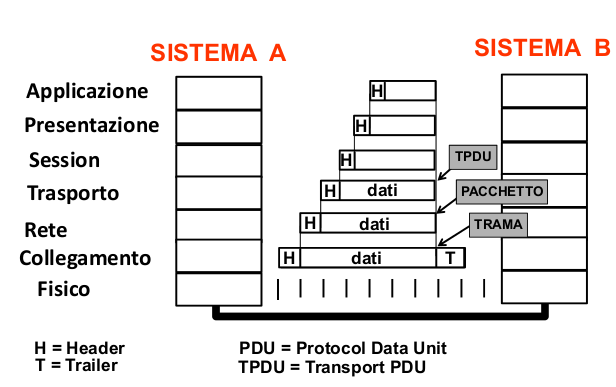
\includegraphics[scale=0.75]{incapsulamento.png}
\end{center}
\section{Stack protocollare TCP/IP}
Il \textbf{TCP/IP} è una famiglia di protocolli attualmente utilizzati in internet. Si tratta di una \textbf{gerarchia di protocolli} costituita da \textbf{moduli interagenti}, ciascuno con funzioni specifiche.
\paragraph{Gerarchia} Con il termine \textbf{gerarchia} s'intende che ciascun protocollo di livello superiore è \textbf{supportato dai servizi forniti dai protocolli di livello inferiore}. Cioè un protocollo a livello \texttt{n} realizza le sue funzionalità grazie ai protocolli a livello \texttt{n-1}.
\begin{multicols}{2}
\subsection{I Livelli}
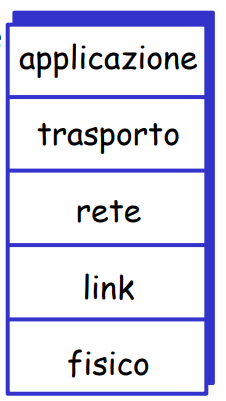
\includegraphics[scale=0.8]{stacktcpip.png}


\columnbreak
Lo stack TCP/IP in origine era intesa come \textbf{quattro livelli software} sovrastanti \textbf{un livello hardware}. Oggi è intesa come semplicemente \textbf{composta da 5 livelli}
\end{multicols}
\pagebreak
\paragraph{Livello Applicativo} Il livello più alto, con il quale interagisce l'utente\\
Identificativi risorse: URL, URI, URN\\
Il web: user agents, http: request, response, connessioni persistenti, GET, POST, PUT, DELETE, status code, proxy server, caching\\
FTP: connessioni dati e di controllo, rappresentazione\\
TELNET\\
Posta elettronica: SMTP, POP3, IMAP\\
DNS e risoluzioni nomi: gerarchia nomi, risoluzione iterativa e ricorsiva, formato pessaggi, nslookup...
\paragraph{Livello Trasporto} Livello al quale si definisce la codifica e il protocollo di trasporto\\
Servizi: mux demux, controllo errore, connectionless\\
TCP: formato segmenti, gestione connessione, controllo flusso e congestione\\
UDP: formato segmenti
\paragraph{Livello Rete} Dove si gestisce l'indirizzamento dei vari host\\
Strato di rete e funzioni\\
Indirizzamentoi IP: classful IPv4, NAT, sottoreti e maschere, classless, CIDR\\
Risoluzione IP e MAC, ARP\\
IPv4: formato datagramma ip, frammentazione\\
Routing IP e istradamento\\
Introduzione IPv6
\paragraph{Livello Link} Trasferimento dati tra elementi di rete vicini\\
Ethernet
\paragraph{Livello Fisico} Bit sul filo
\subsection{strato applicativo}
$https://elearning.di.unipi.it/pluginfile.php/27477/mod_resource/content/2/L03_Applicativo_HTTP.pdf$
...
URI: idetinificativo per una risorsa due tipi\\
	urn\\
	url\\
<authority><path>?<query>\\
authority: nome di dominio che dà risorsa (hostname o indirizzo in notaz puntata)\\

\end{document}